% Options for packages loaded elsewhere
% Options for packages loaded elsewhere
\PassOptionsToPackage{unicode}{hyperref}
\PassOptionsToPackage{hyphens}{url}
\PassOptionsToPackage{dvipsnames,svgnames,x11names}{xcolor}
%
\documentclass[
  letterpaper,
  DIV=11,
  numbers=noendperiod]{scrartcl}
\usepackage{xcolor}
\usepackage{amsmath,amssymb}
\setcounter{secnumdepth}{-\maxdimen} % remove section numbering
\usepackage{iftex}
\ifPDFTeX
  \usepackage[T1]{fontenc}
  \usepackage[utf8]{inputenc}
  \usepackage{textcomp} % provide euro and other symbols
\else % if luatex or xetex
  \usepackage{unicode-math} % this also loads fontspec
  \defaultfontfeatures{Scale=MatchLowercase}
  \defaultfontfeatures[\rmfamily]{Ligatures=TeX,Scale=1}
\fi
\usepackage{lmodern}
\ifPDFTeX\else
  % xetex/luatex font selection
\fi
% Use upquote if available, for straight quotes in verbatim environments
\IfFileExists{upquote.sty}{\usepackage{upquote}}{}
\IfFileExists{microtype.sty}{% use microtype if available
  \usepackage[]{microtype}
  \UseMicrotypeSet[protrusion]{basicmath} % disable protrusion for tt fonts
}{}
\makeatletter
\@ifundefined{KOMAClassName}{% if non-KOMA class
  \IfFileExists{parskip.sty}{%
    \usepackage{parskip}
  }{% else
    \setlength{\parindent}{0pt}
    \setlength{\parskip}{6pt plus 2pt minus 1pt}}
}{% if KOMA class
  \KOMAoptions{parskip=half}}
\makeatother
% Make \paragraph and \subparagraph free-standing
\makeatletter
\ifx\paragraph\undefined\else
  \let\oldparagraph\paragraph
  \renewcommand{\paragraph}{
    \@ifstar
      \xxxParagraphStar
      \xxxParagraphNoStar
  }
  \newcommand{\xxxParagraphStar}[1]{\oldparagraph*{#1}\mbox{}}
  \newcommand{\xxxParagraphNoStar}[1]{\oldparagraph{#1}\mbox{}}
\fi
\ifx\subparagraph\undefined\else
  \let\oldsubparagraph\subparagraph
  \renewcommand{\subparagraph}{
    \@ifstar
      \xxxSubParagraphStar
      \xxxSubParagraphNoStar
  }
  \newcommand{\xxxSubParagraphStar}[1]{\oldsubparagraph*{#1}\mbox{}}
  \newcommand{\xxxSubParagraphNoStar}[1]{\oldsubparagraph{#1}\mbox{}}
\fi
\makeatother


\usepackage{longtable,booktabs,array}
\usepackage{calc} % for calculating minipage widths
% Correct order of tables after \paragraph or \subparagraph
\usepackage{etoolbox}
\makeatletter
\patchcmd\longtable{\par}{\if@noskipsec\mbox{}\fi\par}{}{}
\makeatother
% Allow footnotes in longtable head/foot
\IfFileExists{footnotehyper.sty}{\usepackage{footnotehyper}}{\usepackage{footnote}}
\makesavenoteenv{longtable}
\usepackage{graphicx}
\makeatletter
\newsavebox\pandoc@box
\newcommand*\pandocbounded[1]{% scales image to fit in text height/width
  \sbox\pandoc@box{#1}%
  \Gscale@div\@tempa{\textheight}{\dimexpr\ht\pandoc@box+\dp\pandoc@box\relax}%
  \Gscale@div\@tempb{\linewidth}{\wd\pandoc@box}%
  \ifdim\@tempb\p@<\@tempa\p@\let\@tempa\@tempb\fi% select the smaller of both
  \ifdim\@tempa\p@<\p@\scalebox{\@tempa}{\usebox\pandoc@box}%
  \else\usebox{\pandoc@box}%
  \fi%
}
% Set default figure placement to htbp
\def\fps@figure{htbp}
\makeatother


% definitions for citeproc citations
\NewDocumentCommand\citeproctext{}{}
\NewDocumentCommand\citeproc{mm}{%
  \begingroup\def\citeproctext{#2}\cite{#1}\endgroup}
\makeatletter
 % allow citations to break across lines
 \let\@cite@ofmt\@firstofone
 % avoid brackets around text for \cite:
 \def\@biblabel#1{}
 \def\@cite#1#2{{#1\if@tempswa , #2\fi}}
\makeatother
\newlength{\cslhangindent}
\setlength{\cslhangindent}{1.5em}
\newlength{\csllabelwidth}
\setlength{\csllabelwidth}{3em}
\newenvironment{CSLReferences}[2] % #1 hanging-indent, #2 entry-spacing
 {\begin{list}{}{%
  \setlength{\itemindent}{0pt}
  \setlength{\leftmargin}{0pt}
  \setlength{\parsep}{0pt}
  % turn on hanging indent if param 1 is 1
  \ifodd #1
   \setlength{\leftmargin}{\cslhangindent}
   \setlength{\itemindent}{-1\cslhangindent}
  \fi
  % set entry spacing
  \setlength{\itemsep}{#2\baselineskip}}}
 {\end{list}}
\usepackage{calc}
\newcommand{\CSLBlock}[1]{\hfill\break\parbox[t]{\linewidth}{\strut\ignorespaces#1\strut}}
\newcommand{\CSLLeftMargin}[1]{\parbox[t]{\csllabelwidth}{\strut#1\strut}}
\newcommand{\CSLRightInline}[1]{\parbox[t]{\linewidth - \csllabelwidth}{\strut#1\strut}}
\newcommand{\CSLIndent}[1]{\hspace{\cslhangindent}#1}



\setlength{\emergencystretch}{3em} % prevent overfull lines

\providecommand{\tightlist}{%
  \setlength{\itemsep}{0pt}\setlength{\parskip}{0pt}}



 


\usepackage{parskip}
\usepackage{setspace}
\usepackage{titlesec}
\usepackage{geometry}
\usepackage{microtype}
\usepackage{indentfirst}
\usepackage{ragged2e}
\usepackage{indentfirst}
\setlength{\parindent}{2em}
% Set paragraph indentation and spacing
\setlength{\parskip}{0.5em}

% Adjust margins
\geometry{margin=1in}

% Format section titles
\titleformat{\section}
  {\normalfont\Large\bfseries}{\thesection}{1em}{}
\titlespacing*{\section}{0pt}{3.5ex plus 1ex minus .2ex}{2.3ex plus .2ex}

% Set line spacing
\onehalfspacing

% Improve text justification
\justifying
\usepackage{mathpazo}
\usepackage[T1]{fontenc}
\usepackage[sups,osf]{fbb} % osf (or tosf) for text, not math
\usepackage[scaled=.95]{cabin} % sans serif
\usepackage[varqu,varl]{inconsolata} % sans serif typewriter
\KOMAoption{captions}{tableheading}
\makeatletter
\@ifpackageloaded{caption}{}{\usepackage{caption}}
\AtBeginDocument{%
\ifdefined\contentsname
  \renewcommand*\contentsname{Table of contents}
\else
  \newcommand\contentsname{Table of contents}
\fi
\ifdefined\listfigurename
  \renewcommand*\listfigurename{List of Figures}
\else
  \newcommand\listfigurename{List of Figures}
\fi
\ifdefined\listtablename
  \renewcommand*\listtablename{List of Tables}
\else
  \newcommand\listtablename{List of Tables}
\fi
\ifdefined\figurename
  \renewcommand*\figurename{Figure}
\else
  \newcommand\figurename{Figure}
\fi
\ifdefined\tablename
  \renewcommand*\tablename{Table}
\else
  \newcommand\tablename{Table}
\fi
}
\@ifpackageloaded{float}{}{\usepackage{float}}
\floatstyle{ruled}
\@ifundefined{c@chapter}{\newfloat{codelisting}{h}{lop}}{\newfloat{codelisting}{h}{lop}[chapter]}
\floatname{codelisting}{Listing}
\newcommand*\listoflistings{\listof{codelisting}{List of Listings}}
\makeatother
\makeatletter
\makeatother
\makeatletter
\@ifpackageloaded{caption}{}{\usepackage{caption}}
\@ifpackageloaded{subcaption}{}{\usepackage{subcaption}}
\makeatother
\usepackage{bookmark}
\IfFileExists{xurl.sty}{\usepackage{xurl}}{} % add URL line breaks if available
\urlstyle{same}
\hypersetup{
  colorlinks=true,
  linkcolor={blue},
  filecolor={Maroon},
  citecolor={Blue},
  urlcolor={Blue},
  pdfcreator={LaTeX via pandoc}}


\author{}
\date{}
\begin{document}


\section{Analysis}\label{analysis}

The EEG was recorded using 256 channels. However, certain channels were
identified as potentially noisy or prone to artifact contamination, and
we used only a subset of 204 channels for the analysis. The channels we
used are shown in the figure below (in red are shown discarded
channels).

\begin{figure}

\centering{

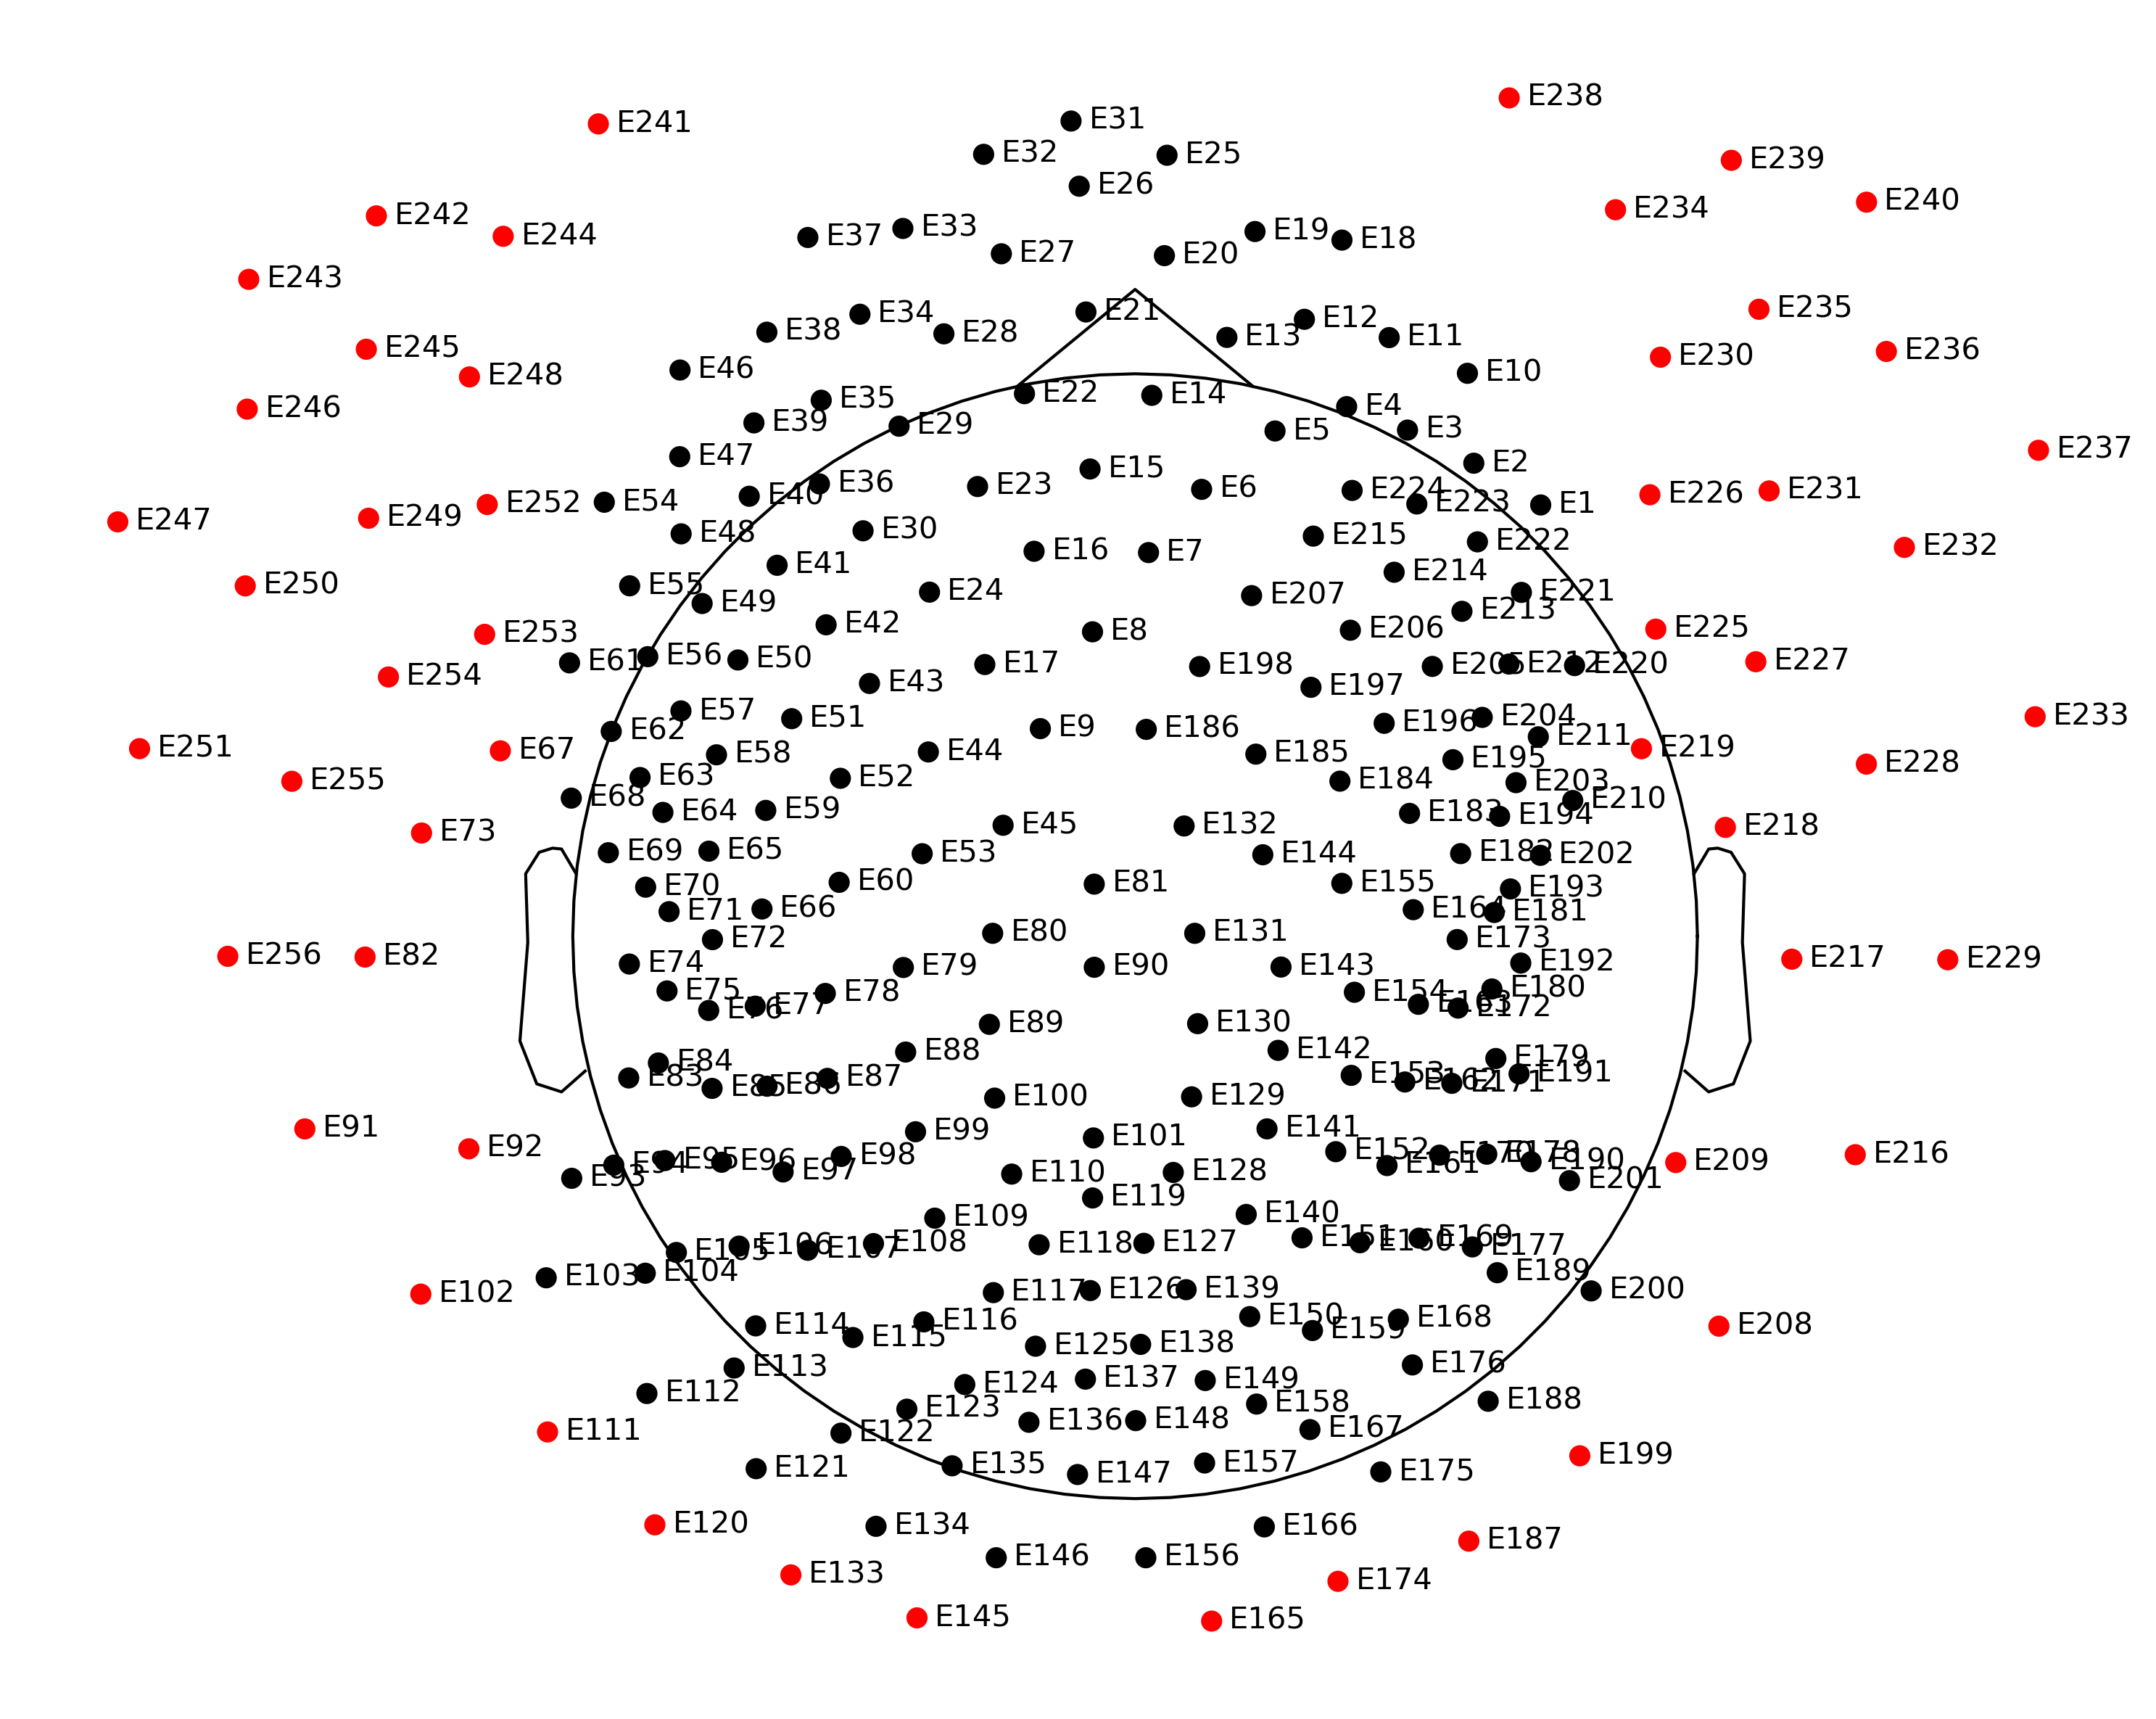
\includegraphics[width=0.8\linewidth,height=\textheight,keepaspectratio]{figures/eeg_montage_plot.png}

}

\caption{\label{fig-channels}Channels used for analysis}

\end{figure}%

\subsection{Preprocessing and EEG
analysis}\label{preprocessing-and-eeg-analysis}

Initially 48 subjects were included into this analysis. EEG data were
analysed using MNE Python (Gramfort et al.
(\citeproc{ref-gramfort2013MEGEEGData}{2013}), version 1.7). Data were
recorded with the resolution 1000 Hz and during the analysis resampled
to 250 Hz and notch filtered at 50 Hz to eleminate line power noise. A
bandpass filter between 1 and 40 Hz was applied using FIR filter. Bad
channels were identified using the Python implementation of the
Preprocessing Pipeline (PREP, Bigdely-Shamlo et al.
(\citeproc{ref-bigdely-shamlo2015PREPPipelineStandardized}{2015})), were
temporarily excluded from analysis and later extrapolated after
performing Independent Component Analysis (ICA).

Dataset was epoched into 5s intervals, with 3s overlap between epochs
(1.5s on each side). The Autoreject library
(\citeproc{ref-jas2017AutorejectAutomatedArtifact}{Jas et al. 2017}) was
used to detect and remove epochs containg huge artifacts (epochs
identified as bad on more than 40\% bad channels were discarded). ICA
was performed on the data using a variable number of the components
determined by capturing 99\% of cumulative variance. The picard method
was employed with the settings
\texttt{fit\_params=dict(ortho=False,\ extended=True)}, which aligns
with \texttt{FastICA} algorithm
(\citeproc{ref-ablin2018FasterIndependentComponent}{Ablin, Cardoso, and
Gramfort 2018}).

The ICA components were visually inspected and those identified as
artifacts were removed. The data were then reconstructed using the
remaining components. For the further analysis, we computed the power
spectral density (PSD) using the Welch method. PSD calculations were
performed for each epoch and then averaged across epochs. The specparam
algorithm (formerly known as fooof,
(\citeproc{ref-donoghue2020ParameterizingNeuralPower}{Donoghue et al.
2020})) was applied with the following parameters: freq\_range = {[}1,
40{]}, peak\_width\_limits = {[}1, 6{]}, min\_peak\_height = 0.15, (?
need to decided if 0.05 or 0.15) peak\_threshold = 2.0, and
max\_n\_peaks = 6.

Similarly to McKeown et al.
(\citeproc{ref-mckeown2023TestretestReliabilitySpectral}{2023}), we
excluded participants with specparam model fits \textless{} 0.9 R2 on
more than 50\% of the channels. Given the above criterium 4 subjects
were identified as those to be exluded from analysis:
\texttt{102\ 103\ 126\ 151}.

\subsection{Results}\label{results}

I manually checked data:

\begin{itemize}
\item
  really good quality 101, 105, 107,112 , 113,114, 115, 122, 123, 127,
  128 , 131, 134, 135, 136, 137, 139 , 142, 143, 144, 149, 152
\item
  good 108, 116, 124, 125, 138 , 145, 146, 148
\item
  medium quality 104, 106, 109 , 110 , 111, 118, 119, 120, 121, 129,
  132, 140, 147, 150
\end{itemize}

\section{Internal discussion}\label{internal-discussion}

\section*{Bibliography}\label{bibliography}
\addcontentsline{toc}{section}{Bibliography}

\phantomsection\label{refs}
\begin{CSLReferences}{1}{0}
\bibitem[\citeproctext]{ref-ablin2018FasterIndependentComponent}
Ablin, Pierre, Jean-François Cardoso, and Alexandre Gramfort. 2018.
{``Faster {Independent Component Analysis} by {Preconditioning With
Hessian Approximations}.''} \emph{IEEE Transactions on Signal
Processing} 66 (15): 4040--49.
\url{https://doi.org/10.1109/TSP.2018.2844203}.

\bibitem[\citeproctext]{ref-bigdely-shamlo2015PREPPipelineStandardized}
Bigdely-Shamlo, Nima, Tim Mullen, Christian Kothe, Kyung-Min Su, and Kay
A. Robbins. 2015. {``The {PREP} Pipeline: Standardized Preprocessing for
Large-Scale {EEG} Analysis.''} \emph{Frontiers in Neuroinformatics} 9
(June). \url{https://doi.org/10.3389/fninf.2015.00016}.

\bibitem[\citeproctext]{ref-donoghue2020ParameterizingNeuralPower}
Donoghue, Thomas, Matar Haller, Erik J. Peterson, Paroma Varma,
Priyadarshini Sebastian, Richard Gao, Torben Noto, et al. 2020.
{``Parameterizing Neural Power Spectra into Periodic and Aperiodic
Components.''} \emph{Nature Neuroscience} 23 (12): 1655--65.
\url{https://doi.org/10.1038/s41593-020-00744-x}.

\bibitem[\citeproctext]{ref-gramfort2013MEGEEGData}
Gramfort, Alexandre, Martin Luessi, Eric Larson, Denis A. Engemann,
Daniel Strohmeier, Christian Brodbeck, Roman Goj, et al. 2013. {``{MEG}
and {EEG} Data Analysis with {MNE-Python}.''} \emph{Frontiers in
Neuroscience} 7 (December).
\url{https://doi.org/10.3389/fnins.2013.00267}.

\bibitem[\citeproctext]{ref-jas2017AutorejectAutomatedArtifact}
Jas, Mainak, Denis A. Engemann, Yousra Bekhti, Federico Raimondo, and
Alexandre Gramfort. 2017. {``Autoreject: {Automated} Artifact Rejection
for {MEG} and {EEG} Data.''} \emph{NeuroImage} 159 (October): 417--29.
\url{https://doi.org/10.1016/j.neuroimage.2017.06.030}.

\bibitem[\citeproctext]{ref-mckeown2023TestretestReliabilitySpectral}
McKeown, Daniel J, Anna J Finley, Nicholas J Kelley, James F Cavanagh,
Hannah A D Keage, Oliver Baumann, Victor R Schinazi, Ahmed A Moustafa,
and Douglas J Angus. 2023. {``Test-Retest Reliability of Spectral
Parameterization by 1/ {\emph{f}} Characterization Using
{\emph{SpecParam}}.''} \emph{Cerebral Cortex}, December, bhad482.
\url{https://doi.org/10.1093/cercor/bhad482}.

\end{CSLReferences}




\end{document}
